%%%%%%%%%%%%%%%%%%%%%%%%%%%%%%%%%%%%%%%%%%%%%%%%%%%%%%%%%%%%%%%%%%%%%%%%%%%%%%%%
\documentclass[12pt,papel,twoside]{ibtesis}
%\documentclass[12pt,screen,twoside,pagebackref]{ibtesis}
%\documentclass[12pt,papel,singlespace,oneside]{ibtesis}
% \documentclass[12pt,papel,preprint,singlespace,oneside]{ibtesis}
%%%%%%%%%%%%%%%%%%%%% Paquetes extra %%%%%%%%%%%%%%%%%%%%%%%%%%%%%%%%%%%%%%%%%%%
% Por conveniencia: aqu\'{\i} puede cargar todos los paquetes y definir los comandos 
% que necesite
\usepackage{ibextra}
\usepackage{subfig} %para poner varias imagenes en una sola figura
\usepackage{url} %para citar páginas web
\usepackage{notoccite}
\usepackage{verbatim}
\usepackage{enumerate}
\usepackage{listings}
\usepackage{hyperref}
\usepackage[table,xcdraw]{xcolor}
%\usepackage{graphicx}
%\nofiles
%%%%%%%%%%%%%%%%%%%%%%%%%%%%%%%%%%%%%%%%%%%%%%%%%%%%%%%%%%%%%%%%%%%%%%%%%%%%%%%%
%%%%%%%%%%%%%%%%%%%%% Informacion sobre la tesis %%%%%%%%%%%%%%%%%%%%%%%%%%%%%%%
\title{Anisotropía de la Microestructura de Aleaciones Metálicas por Difracción de Luz Sincrotrón}
\author{Mg. Emanuel Alejandro Benatti}
\director{Dr. Raúl Eduardo Bolmaro}
\carrera{Tesis Doctorado en F\'{\i}sica}
\grado{Doctorando}
\laboratorio{Física y Micromecánica de materiales heterogéneos \\ Instituto de Física Rosario}
%\palabrasclave{DETECTOR, SUPERCONDUCTOR, MgB$_{2}$, NEUTRÓN}
%\keywords{detector, superconductor, MgB$_{2}$, neutron}
% Si queremos poner la fecha manualmente:
% \date{Diciembre de 2099}

%%%%%%%%%%%%%%%%%%%%%%%%%%%%%%%%%%%%%%%%%%%%%%%%%%%%%%%%%%%%%%%%%%%%%%%%%%%%%%%%
%\titlepagefalse % Si no quiere compilar la portada descomente esta linea
%\includeonly{apendices} % Compilar s\'{o}lo estos archivos 
%\graphicspath{{figs/}} % Lugar donde encontrar las figuras generales (se puede poner uno en cada cap{\'{\i}}tulo)
%%%%%%%%%%%%%%%%%%%%%%%%%%%%%%%%%%%%%%%%%%%%%%%%%%%%%%%%%%%%%%%%%%%%%%%%%%%%%%%%


\begin{document}

% Dentro del environment 'preliminary' va:
% la dedicatoria, resumen, abstract, indices

\begin{preliminary}

% Escriba su dedicatoria
\dedicatoria{
A mi familia\\
A mis amigos\\
y a todos los que se lo merecen \\
por merecerlo. \\
}

%%% \'{I}ndices %%%%
%\begin{abreviaturas}
%    \printnomenclature
%\end{abreviaturas}

\tableofcontents                %\'{I}ndice

\begin{resumen}%
  En este trabajo se estudia la viabilidad de utilizar films del supuerconductor MgB$_2$, que tiene una temperatura crítica alrededor de 39\,K, para construir un detector de neutrones térmicos y fríos. El objetivo es aprovechar el calor generado por la reacción $^{10}$B$(n,\alpha)^6$Li que tiene una sección eficaz de 3800\,barns para neutrones térmicos y libera una energía de aproximadamente 2.3\,MeV. El calor producido por la reacción produce una supresión momentánea de la superconductividad, lo que produce una señal que permite registrar la captura de un neutrón. Se realizaron simulaciones de las trayectorias de los productos de la reacción en el MgB$_2$ para estimar las dimensiones del detector que permitan maximizar su señal, sensibilidad y eficiencia, y que minimicen el tiempo de respuesta, al tiempo que se estimó que la energía de la reacción se deposita en un volumen de unos pocos micrómetros cúbicos. Cálculos y simulaciones hechas con el software comercial de elementos finitos COMSOL MULTIPHYSICS llevaron a la conclusión de que para poder detectar eficientemente neutrones con el MgB$_2$, resulta necesario construir un cable que tenga un ancho no mayor a un micrón y un espesor no mucho mayor a los 200\,nm. Dimensiones mayores incrementan la probabilidad de captura de un neutrón pero reducen drásticamente la señal y la sensibilidad del detector, además de que dificultan el control de la temperatura del mismo.

Fueron realizadas simulaciones en las que se acopló la física del comportamiento térmico y eléctrico del detector, y se observó que si el mismo es operado con corrientes lo suficientemente bajas, la señal y el tiempo de respuesta del detector no se modifican, y que tiene un tiempo de respuesta de algunos nanosegundos cuando el espesor del cable es de 200\,nm. También se llevaron a cabo simulaciones intentando regular la temperatura del detector simplemente variando la tensión aplicada al mismo, pero el resultado fue que eso no es posible desde el punto de vista práctico, ya que para regular la temperatura del detector en el rango de interés, es preciso aplicar tensiones que llevan a que circulen corrientes enormes por el cable de MgB$_2$. La conclusión extraída de este cálculo fue que el detector va a requerir un mecanismo adicional para controlar su temperatura. También se concluyó que por razones de estabilidad en el control de la misma, es conveniente operar al detector a tensión constante, en vez de hacerlo a corriente constante.

En conjunto con el trabajo de las simulaciones se intentó crecer films de MgB$_2$ por medio de dos técnicas diferentes, una utilizando un método ex-situ que requrió temperaturas del orden de los 700\,$^{\circ}$C, y otra consistente en un método in-situ que requería temperaturas iban de los de 500\,$^{\circ}$C hasta temperatura ambiente.

La primera técnica de crecimiento consistió en depositar films de B por evaporación para luego recocer los mismos junto con pastillas de MgB$_2$ bulk en ampollas de cuarzo. Se lograron fabricar films de un espesor de algunos cientos de nanómetros, cuyas curvas de magnetización, medidas en un magnetómetro SQUID, presentaron irreversibilidades en un ciclo \textit{Zero Field Cooling - Field Cooling} compatibles con la formación de una fase superconductora. Sin embargo, siguiendo este método no se pudo conseguir fabricar films con una transición superconductora lo suficientemente estrecha como para poder fabricar el detector, lo que probablemente se debió a que el sustrato reaccionaba con el film debido a las elevadas temperaturas del recocido.

La segunda técnica de crecimiento de films de MgB$_2$ explorada en este trabajo fue la de crecimiento directo de films por sputtering, a partir de un blanco de MgB$_2$ obtenido comercialmente. Se realizaron estudios de difracción de rayos X que no mostraron la formación de la fase MgB$_2$. Un estudio de la composición de los films crecidos fue realizado utlizando espectroscopía de rayos X caracterísiticos (EDX) y retrodispersión de Rutherford (RBS). Ambos estudios mostraron que los films crecidos tienen un exceso de B, lo que probablemente sea la causa de que no sean superconductores, tal como mostraron las mediciones de magnetización realizadas sobre las muestras. Se decidió intentar recocer los films crecidos con pastillas de Mg, en busca de mejorar la proporcion B/Mg de los films utilizando una temperatura de recocido más baja que la empleada con los films crecidos por evaporación. El recocido logró una mejora en las propiedades de transporte de las muestras, ya que pasaron de ser aislantes a ser semiconductoras, pero no se pudo observar la formación de fases superconductoras, ni en mediciones de magnetización, ni en mediciones de transporte, lo que consituye un indicio de que los films no lograron incorporar la cantidad suficiente de Mg como para volverse superconductores. Esto último se deba probablemente a que la temperatura de recocido no fue lo suficientemente alta como para permitir la difusión de la cantidad necesaria de Mg a través del film.
\end{resumen}

\begin{abstract}%
	In this paper we study the feasibility of using films of the superconductor MgB$_2$ with a critical temperature of 39\,K, to build a cold neutron and thermal neutron detector. The aim is to use the heat generated by the reaction $^{10}$B$(n,\alpha)^6$Li which has a cross section of 3800\,barns for thermal neutrons and releases an energy of approximately 2.3\,MeV. The heat produced by the reaction causes a partial destruction of superconductivity. One then notices the appearance of a single neutron by the electric resistance variation of the MgB2 thin film. Simulations of the trajectories of the reaction products in the MgB$_2$ were performed for estimating the optimal detector dimensions. Calculations and simulations with the commercial software COMSOL Multiphysics led to the conclusion that in order to efficiently detect neutrons with MgB$_2$, is necessary to build a cable that has a width no greater than one micron and a thickness not much greater than 200\,nm. Larger dimensions increase the probability of neutron capture but drastically reduces the produced signal and the detector sensitivity, plus it difficult the temperature control of the device.

	Simulations were also conducted coupling the physics of the thermal and electrical behavior of the detector, and it was found that if it is operated with a small bias-current, the detector's signal and response time are not changed. Calculations showed that the detector has a response time of few nanoseconds for a wire 200\,nm thick. Simulations were carried out trying to regulate the temperature of the detector by varying the bias tension, but it was found that this is not a viable option from a practical standpoint, as to regulate the temperature of the detector in the range of interest, it is necesary to apply voltages that lead to large currents circulating through the detector. This implied that the construction of the detector will require an additional mechanism to control its temperature. It was also found that for reasons of stability in temperature control, it is desirable to operate the detector voltage-biased instead of current-biased.

	In addition with the simulations, growth of MgB$_2$ films was attempted by two different means, one using an ex-situ method requiring temperatures around 700\,$^{\circ}$C, and an in-situ method requiring temperatures of 500\,$^{\circ}$C down to room temperature.

	The first technique consisted on growing of boron films by evaporation and a post-annealing process with a bulk MgB$_2$ sample in a quartz tube. We managed to make 200\,nm thick films, and perform magnetization measurements in a SQUID magnetoteter. Irreversibilities shown in a Zero Field Coolig - Field Coolig magnetization measurement were compatible with the formation of a superconducting phase. However, it wasn't possible to obtain films with a sharp superconducting transition, as it's needed to build the detector. This is probably the result of a chemical reaction between substrate and the film due to the high annealing temperatures.

  The second technique explored in this work was the direct growth of MgB$_2$ films by sputtering. To this end a commercial MgB$_2$ target was used. Studies performed by X-ray diffraction did not show the formation of the MgB$_2$ crystalline phase. We also studied the composition of the films by electron dispersive X-ray analisys (EDX) and Rutherford backscattering (RBS). Both studies showed that films are grown with an excess of B, which is probably the reason why they are not superconducting, as was observed by magnetization measurements. Films were annealed with Mg pellets, seeking to increase the amount of Mg in the films, using lower annealing temperatures than those used with the films grown by evaporation. Samples showed an improvement in their transport properties after the annealing, as they went from being insulating to semiconductonducting. However no formation of a superconducting phase was observed, neither in magnetization measurements or in electrical resistance measurements. This is probably due to the low annealing temperature, which did not allow the diffusion of the required amount of Mg through the film.
\end{abstract}

%%% Local Variables: 
%%% mode: latex
%%% TeX-master: "template"
%%% End: 

\end{preliminary}


% Podemos usar cualquiera de los dos comandos: \input o \include para incluir el texto
\chapter{Introducci\'on}
\graphicspath{{./figs/01_intro/}}
\chapterquote{La destrucción es obra de una tarde. La creación es obra de una vida.}{Kamahl, acólito druida}
\section{Motivación}\label{S:motivacion}
\cite{Mainprice2011}
\section{Difracción de Rayos X}\label{S:DRX}
Los rayos X son una herramienta de vital importancia para el estudio de los materiales cristalinos. 
En la difracción de Rayos X (DRX), un haz monocromático de de rayos X de longitud de onda $\lambda$ incide sobre una dada muestra (Fig. \ref{fig:Bragg}). 
Si el cristal es infinito y está libre de cualquier tipo de distorsiones, para una dada familia de planos ${hkl}$, habrá interferencia constructiva para los haces salientes que cumplan con la condición de Bragg[ref]:

Esto esta medio medio, hay que hablar de que los cristales estan en arreglos periodicos de atomos

\begin{equation}
  2 \ d_{hkl} \ \sin(\theta_{B}) \ = \ n \ \lambda
  \label{eq:Bragg}
\end{equation}
\noindent
siendo $d_{hkl}$ la distancia interplanar de la familia de planos $\{hkl\}$, 2$\theta_{B}$ el ángulo formado entre el haz incidente y el haz reflejado y $n$ el número de orden de difracción. 

Hay que pensar en el planteo mas riguroso, usando los vectores K, porque lo voy a necesitar para explicar williamson hall

\nomenclature{$\lambda$}{Longitud de onda}
\nomenclature{$d_{hkl}$}{Distacia interplanar para la familia de planos $hkl$}
\nomenclature{$\theta_B$}{Ángulo de Bragg}
\nomenclature{XRD}{Difracción de Rayos X}
\begin{figure}[htb!]
  \centering
  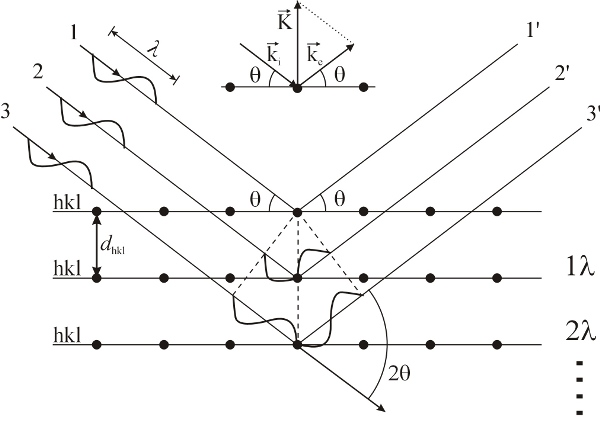
\includegraphics[width=\imsize]{BraggLaw}
  \caption{Ley de Bragg}
  \label{fig:Bragg}
\end{figure}

Una consecuencia de la ley expresada en la Ec. \ref{eq:Bragg} es que para un cierto haz incidente habrá reflexiones cuyas distribución de intensidades serán funciones deltas de Dirac[ref], con intensidad infinita para el ángulo $\theta_{B}$ e intensidad nula para los ángulos $\theta$ que no cumplan con la condición de Bragg. Como resultado, los "picos" de difracción tendrán además un ancho nulo. 
Si, como ocurre en la práctica, el número de planos que contribuyen a la reflexión es finito, la distribución angular de intensidades tendrán un ancho y altura finitos, y lo mismo ocurrirá si la red de átomos tiene distorsiones, es decir, si los átomos no se encuentran en un arreglo perfectamente periódico. 
En un experimento de DRX real aparecerán además otras contribuciones que ensancharán los picos de difracción. 
Por un lado el haz incidente no será puntual ni estará constituido por haces completamente paralelos, sino que tendrá de un tamaño finito y estará comprendido entre haces que tendrán cierta divergencia angular. 
Además, el haz no será completamente monocromático, sino que estará inegrado por rayos X con longitudes de onda en un intervalo $(\lambda \ \pm \ \Delta \lambda)$. 
Todos estos factores cotribuirán a que haya haces difractados en las vecindades de $\theta_{B}$, aumentando el ancho de los picos de difracción, y serán parte crucial de la discusión en los capítulos siguientes, ya que el ensanchamiento de los picos provee información sobre la microestructura de los materiales.

\subsection{Estudios de ancho de pico}\label{SS:DRX-LPA}
Si no se tienen en cuenta los diferentes efectos instrumentales se puede afirmar que, a partir del estudio del ensanchamiento y la forma de los perfiles de intensidad de los picos de medidos en un experimento de DRX, es posible obtener información acerca de la cantidad y tipo de defectos presentes en un material, así como información microestructural como el tamaño promedio de los dominios coherentes de difracción. 
Al conjunto de t\'ecnicas y m\'etodos del campo de la cristalografía que utilizados para obtener este tipo de información se los conoce como Estudio de Ancho de Pico, o LPA, por sus siglas en inglés (Line Profile Analysis).
Aunque el término LPA fue acuñado muchos años después, la técnica, aunque rudimentaria, es tan antigua como los primeros experimentos de DRX, y fue implementada independientemente por Hull en Estados Unidos y Debye y Scherrer en Alemania. Mientras investigaba el tamaño de partículas de oro y plata en sistemas coloidales, Scherrer incluyó la ecuación que luego llevaría su nombre[ref]:

\begin{equation}
  H \ = \ 2 \sqrt{\frac{\ln(2)}{\pi}} \ \frac{\lambda}{L \ \cos(\theta_B)}
  \label{eq:Scherrer}
\end{equation}
\noindent
Donde $H$ denota el ancho del pico a la mitad de su intensidad máxima, $L$ es la longitud característica de la cristalita y el factor numérico se usa para convertir $H$ al ancho integral del pico, suponiendo que el mismo tiene forma de gaussiana. 
Los trabajos que siguieron se dedicaron a mejorar las estimaciones de tamaño y forma de las cristalitas. 
En el año 1938 [ref] Jones señaló que el perfil de intensidades medido en un experimento de DRX, $I_{exp}$ es la convolución del perfil $I_{muestra}$ que se obtendría de la muestra y el debido a todos los efectos instrumentales, $I_{inst}$, es decir:
\begin{equation}
  I_{exp} \ = \ I_{muestra} \ \otimes \ I_{inst}
  \label{eq:conv}
\end{equation}
\noindent
De esta manera, Jones logró remover las contribuciones de las líneas $K\alpha_2$ de la radiación del cobre en las mediciones de tamaño de cristalita.


\nomenclature{$H$ o $FWHM$}{Ancho de pico a media altura. También abreviado como FWHM por sus siglas en inglés (Full Witdth at Half Maximum).}
\nomenclature{$L$}{Longitud característica de la cristalita.}

Frase de Warren?
Definicion de macro, micro, meso, nano estructura?
Diferencia entre cristalita y tamaño de grano
Definicion de defectos, dislocaciones, maclas, fallas de apilamiento, bordes de grano
Separacion, al menos en la nomenclatura de familia de planos, planos, direcciones familia de direcciones

Hay que hablar de los principios de medicion, rayos X de laboratorio y de sincrotron
Estudio de ancho de pico, Langford, Williamson Hall, Warren Averbach y CMWP

\section{Difracción de electrones retro difundidos}\label{S:EBSD}
Cómo se mide y cómo se pueden relacionar las magnitudes de EBSD con las de RX
Que permite y que no permite ver en comparacion con RX

¿Hablo de TEM?
 
\section{Textura cristalográfica}\label{S:Text}
Definicion de textura, relacion con los procesos de deformacion y la microestructura.
ODF: definicion y obtencion a partir de RX y EBSD. Diferencias de los dos métodos.

\subsection{FDO y FDO generalizada}\label{SS:ODF}
Relacion entre la ODF y la ODF generalizada. Relacion de FWHM y energía de deformacion.

\section{Revisión bibliográfica y estado del arte}\label{S:RB}

\section{Organización de la tesis}\label{S:Org}

\chapter{Materiales y métodos}\label{C:Materiales}
\graphicspath{{./figs/02_Mat/}}
\section{Experimentos de difracción de rayos X}\label{S:MatXRD}
Buena parte del trabajo de esta tesis se centró alrededor de los experimentos de difracción de rayos X.
En particular, la mediciones se hicieron empleando la geometría de transmisión, también llamada de Debye-Scherrer, utilizando radiación sincrotrón.
La facilidad en la que se trabajó fue PETRA III, cuya fotografía puede verse en la Fig. \ref{fig:desyfoto}, y está ubicada en el complejo DESY, en la ciudad de Hamburgo, Alemania\cite{desy}.

\begin{figure}[!htb] 
  \centering
  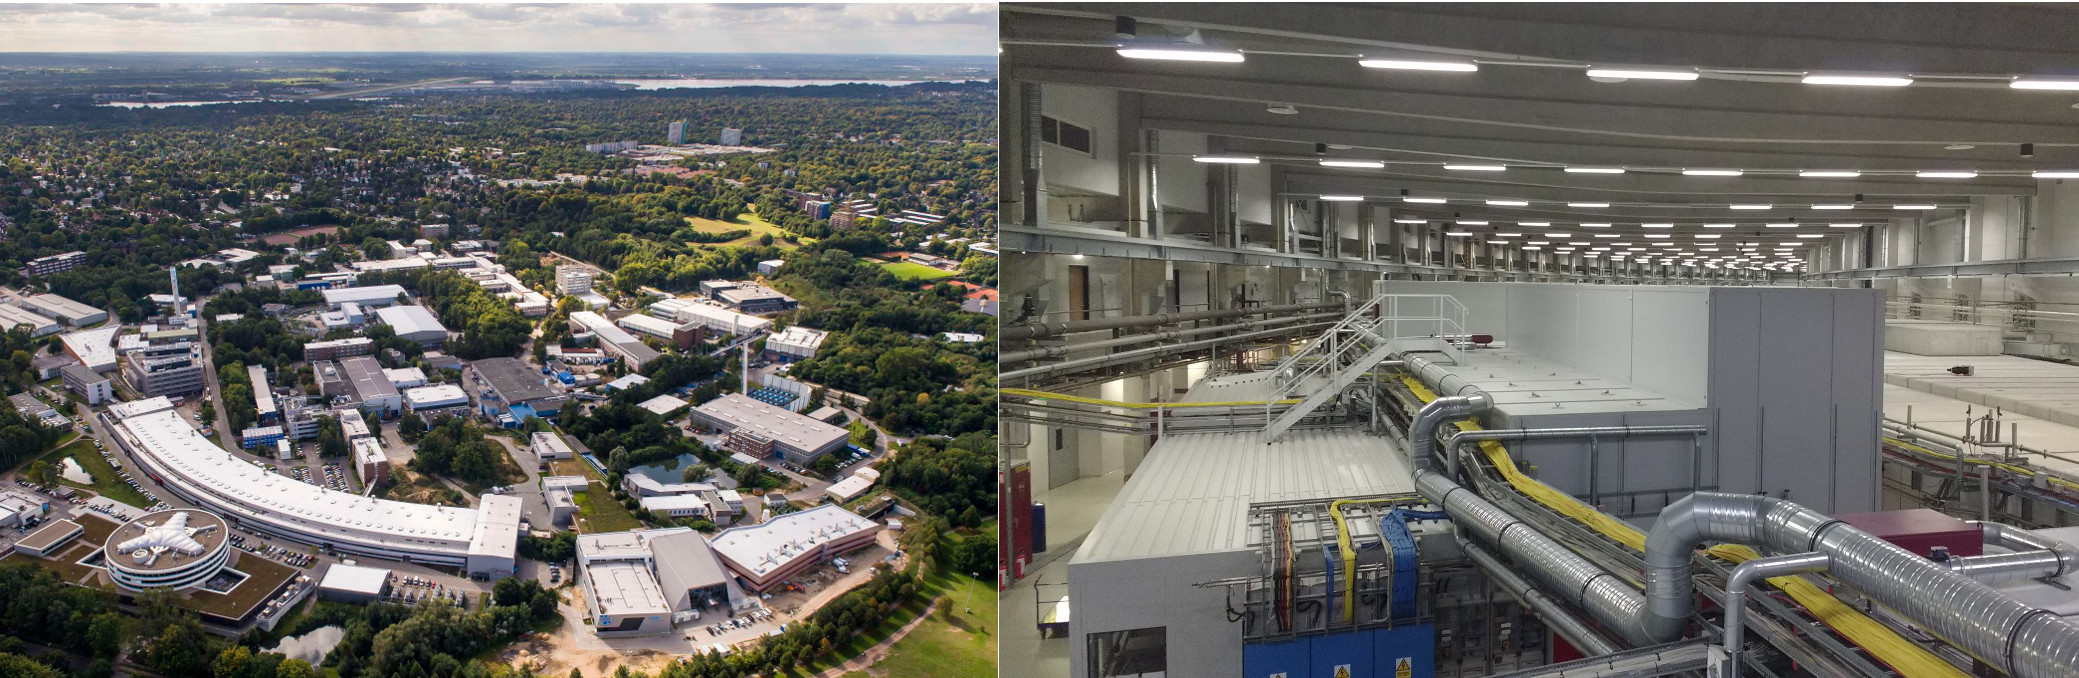
\includegraphics[width=\textwidth]{desy}
  \caption{Fotografías del exterior e interior de la facilidad PETRA III, en DESY. Imágenes obtenidas de \cite{desy}.}
  \label{fig:desyfoto}
\end{figure}

En los experimentos de transmisión realizados, se hizo incidir un haz de rayos\,X con $\lambda \ \approx \ 0.0142$\,nm sobre una muestra, como está esquematizado en la imagen de la Fig. \ref{fig:transmision}. 

Como resultado de la interacción elástica entre el haz incidente y el material, diferentes haces con la misma energía que el incidente, son dispersados por diferentes familias de planos en ángulos que están dados por la Ley de Bragg \ref{eq:Bragg}.
Para una dada familia de planos $\{hkl\}$ todos los haces difractados están comprendidos en un cono, que al interceptar el detector forman un círculo, denominado anillo de Debye, y la intensidad del haz difractado a lo largo de largo del anillo de Debye está determinada por la cantidad de planos cristalinos en condición de difracción para esa dada orientación de la muestra.

En la configuración que se muestra en la Fig. \ref{fig:transmision} la muestra se colocó en un porta-muestra que permitía la alineación con el haz y el detector, y le daba a la misma la libertad de girar alrededor de un eje vertical que pasaba por su centro.
La muestra giraba gracias a un motor paso a paso y que permitía rotarla con una precisión de 5\,$^{\circ}$ por paso.
Para obtener una caracterización completa de la textura de la muestra, fue necesario rotar la misma un rango de 180\,$^{\circ}$, lo que sumado al paso de la rotación significó que por cada muestra se obtuvieron 37 anillos de Debye.

\begin{figure}[!htb]
  \centering
  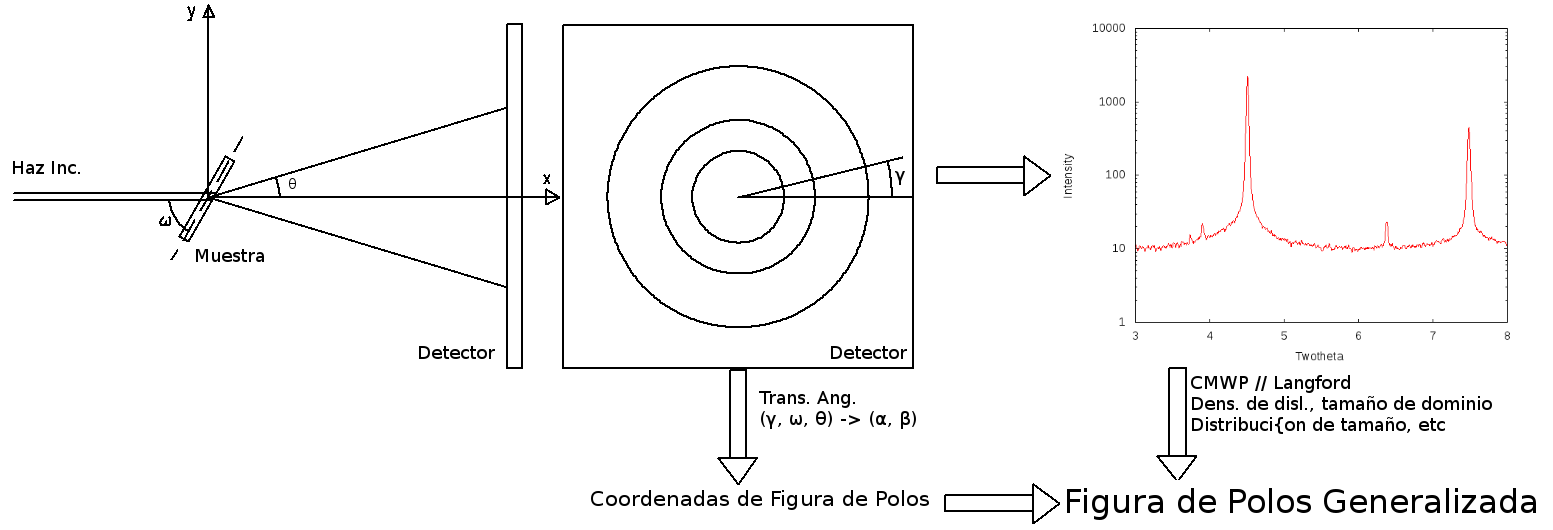
\includegraphics[width=\textwidth]{process}
  \caption{Esquema básico del proceso de medición y análisis de datos. Las mediciones se realizaron empleando una geometría de transmisión, para diferentes rotaciones $\omega$ de la muestra. Por cada posición de la muestra se registraron una serie de anillos de Debye, a partir de los cuales se extrajeron porciones radiales, con las que se construyeron difractogramas que luego fueron procesados siguiendo diferentes modelos de LPA. A partir de estos resultados, y realizando la conversión adecuada de las coordenadas de laboratorio a las coordenadas del sistema de referencia del cristal, se construyeron figuras de polos y figuras de polos generalizadas.}
  \label{fig:transmision}
\end{figure}

\nomenclature{LPA}{Análisis de ancho de pico}

El haz que incidente tenía un tamaño de 100\,$\mu$m x 100\,$\mu$m, lo que permitía obtener una gran resolución sobre la micro-estructura del material.
Las muestras empleadas eran varillas aproximadamente cuadradas, con su eje colocado verticalmente, es decir, paralelo al eje de giro.

El ancho de las varillas era de entre 2\,mm y 5\,mm, y se tuvo especial cuidado durante la alineación de que el haz esté completamente adentro de la muestra en todo el rango de rotación de la misma. 

Las muestras fueron cortadas a partir de las barras originales empleando una sierra de punta de diamante, para luego se pulida con papel de lija hasta que se logró el espesor final.

Se utilizó un detector de estado sólido Mar345 de forma cuadrada, con una grilla de 3450\,píxeles x 3450\,píxeles, de 100\,$\mu$m x 100\,$\mu$m cada uno.
El detector se colocó 1081\,mm detrás de la muestra, y los tiempos de detección se modificaron de acuerdo a la intensidad de salida del haz y la absorción de la muestra, de modo de que las intensidades máximas siempre estén cerca del número máximo de cuentas adquiribles por el detector.

De cada medición se extrajeron 37 imágenes, cada una de las cuales contaba con conjuntos de 5 a 7 anillos de Debye, dependiendo de la muestra.
De cada imagen se extrajeron porciones radiales de ancho angular de 5\,$^{\circ}$ a partir de las cuales se construyeron 72 difractogramas.
El conjunto de 72 x 37 = 2664 difractogramas fue analizado utilizando diferentes modelos de LPA, pero hubo dos modelos sobre los que se hizo especial foco: el de Langford (Sec. \ref{SS:Langford}) y el CMWP (Sec. \ref{SS:CMWP}), y de cada modelo empleado se extrajo diferente información sobre la micro-estructura de la muestra.

Cada pico de cada difractograma quedaba identificado por su ángulo de Bragg $\theta_B$, su coordenada angular $\gamma$ en el anillo de Debye y la rotación de la muestra $\omega$ cuando se realizó la medición, por lo que la información micro-estructural que se extraía del ancho de los picos era susceptible de ser graficada empleando figuras de polos, de la misma manera que se grafican las figuras de polos.
Para construir figuras de polos a partir de las mediciones realizadas fue preciso transformar las coordenadas de los picos en el sistema de laboratorio $(\omega, \gamma, \theta_B)$ a la del sistema de referencia del cristal $(\alpha, \beta)$, para lo cual se empleó la matriz de rotación ya calculada por Bunge y Klein\cite{Bunge1996}.
La misma expresión fue empleada para generar las figuras de polos generalizadas.

\subsection{Contribuciones instrumentales al ancho de pico}\label{SS:inst}
Para poder realizar un análisis micro-estructural preciso a partir de mediciones de ancho de pico, es necesario dar cuenta del ancho instrumental del equipo empleado.
Se define como ancho instrumental al ensanchamiento que se observa alrededor de los picos de Bragg, y que es independiente de la micro-estructura de la muestra estudiada.
Para medir el ancho instrumental se emplean muestras patrones, es decir, muestras que poseen una geometría similar a la de las muestras a estudiar y que no poseen ensanchamiento (o poseen un ensanchamiento muy pequeño) debido a factores micro-estructurales, como ser tensiones internas y tamaño de grano.
También es necesario que los patrones instrumentales no posean ningún tipo de textura.
Para las mediciones de este trabajo se utilizó un polvo de LaB$_6$ como patrón instrumental.

En la Fig. \ref{fig:LaB6vsGamma} puede verse el ancho de uno de los picos del patrón de LaB$_6$ a lo largo del anillo de Debye para tamaños de haz de 100\,$\mu$m x 100\,$\mu$m y 500\,$\mu$m x 500\,$\mu$m.
Notar que no sólo el ancho instrumental se reduce con el tamaño del haz, sino que además existe una variación del mismo a medida que se recorre el anillo de Debye, con mínimos en 90\,$^{\circ}$ y 270\,$^{\circ}$, un máximo local en 180\,$^{\circ}$ y un máximo absoluto en 0\,$^{\circ}$/360\,$^{\circ}$, y que esta variación se reduce también con el tamaño del haz, aunque nunca desaparece del todo.

\begin{figure}[!htb]
  \centering
  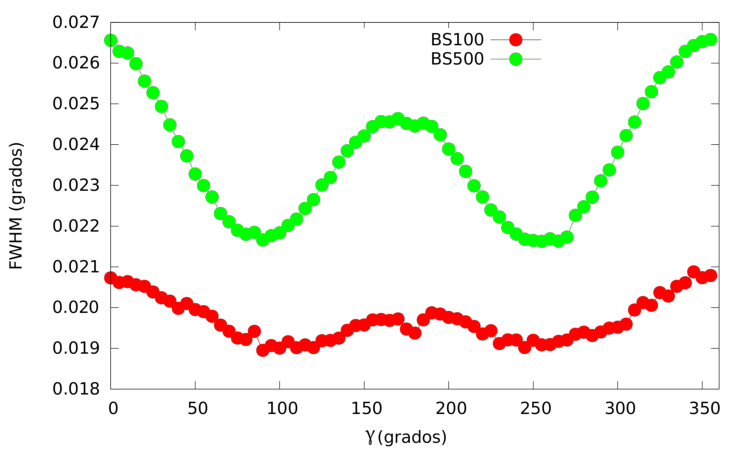
\includegraphics[width=0.95\textwidth]{LaB6_1mm_FWHMvsGammavsBS.pdf}
  \caption{Variación del ancho instrumental como función del ángulo $\gamma$ a lo largo del anillo de Debye para diferentes tamaños del haz incidente. Puede apreciarse que reducir el tamaño del haz reduce el valor promedio del ancho instrumental. También puede verse que el ancho instrumental no es uniforme a lo largo de todo el anillo de Debye, sino que se presentan oscilaciones que también se reducen al reducir el área del haz incidente.}
  \label{fig:LaB6vsGamma}
\end{figure}

La razón de esta oscilación en el ancho instrumental se debe a la divergencia del haz de rayos X\cite{Wcislak2002} y esta es una fuente de errores sistemáticos bastante común en los experimentos realizados con geometrías de transmisión, aunque su presencia suele quedar enmascarada cuando el ensanchamiento de los picos debido a la micro-estructura es mucho más grande que el instrumental.

En casos donde el ensanchamiento de la muestra no es tan grande, la contribución de la divergencia del haz se puede apreciar fundamentalmente como una asimetría izquierda-derecha en las figuras de polos generalizadas de ancho de pico, en el que el lado derecho e izquierdo tienen la misma estructura general, pero el derecho tiene un valor promedio visiblemente más alto, como se ve en la Fig. \ref{fig:IF75NoSym}-a.

\begin{figure}[!htb] 
  \centering
  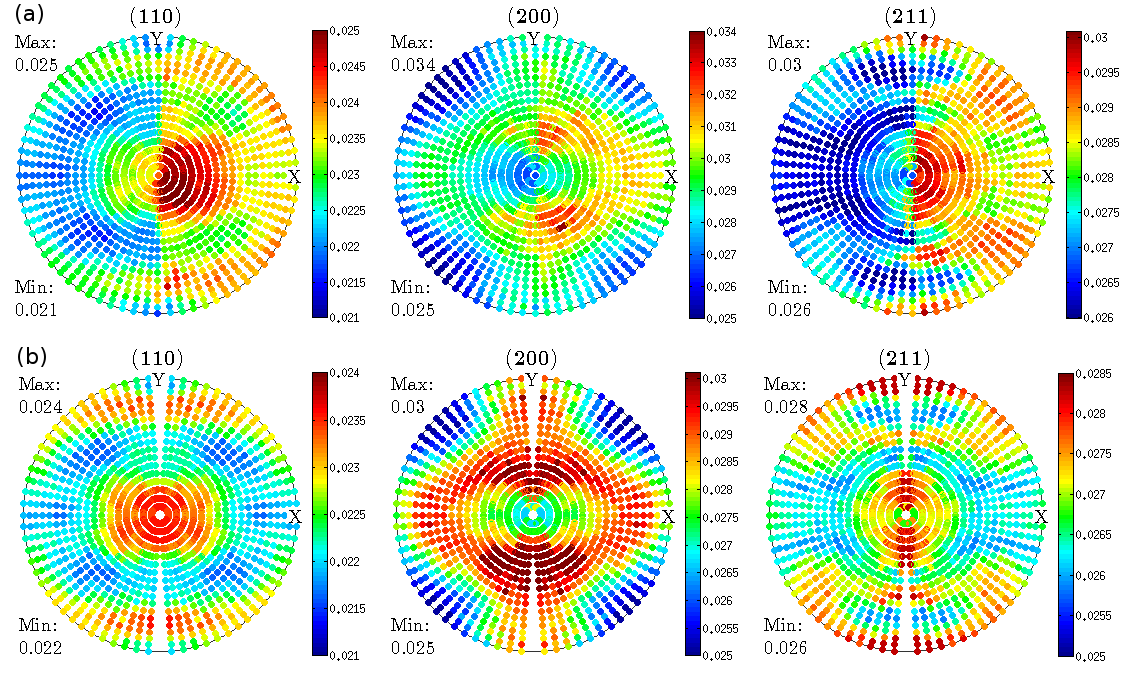
\includegraphics[width=0.95\textwidth]{IF75_SymnoSym}
  \caption{Efecto de la contribución de la divergencia del haz al ancho de pico medido. En la parte (a) de la figura pueden observarse las figuras de polos generalizadas de ancho de pico de una muestra de acero libre de intersticiales. Se observa que los datos a la derecha tienen una estructura similar a la de los de la izquierda, sólo que con un valor medio un poco más alto. En la parte (b) de la figura se simetrizó la figura de polos a partir de reflejar los datos de la izquierda a la derecha.}
  \label{fig:IF75NoSym}
\end{figure}

Inicialmente se intentó hacer una sustracción del ancho instrumental a partir de ajustar el patrón de LaB$_6$ y ajustar la componente Lorentziana y Gaussiana de cada uno de los picos empleando la expresión de Caglioti\cite{Caglioti1958}, para luego restar el ancho instrumental al medido en los experimentos:
\begin{align}
  H_L^{micr} & = H_L^{exp} \ - \ H_L^{inst} \nonumber \\
  (H_G^{micr})^2 & = (H_G^{exp})^2 \ - \ (H_G^{inst})^2 
  \label{eq:instrumental}
\end{align}
\noindent
donde $H_i^{micr}$, $H_i^{exp}$ y $H_i^{inst}$ representan los ensanchamientos micro-estructurales, experimentales e instrumentales respectivamente, y la substracción que se hace es la que corresponde atendiendo al carácter lorentziano o gaussiano de los picos.

Para hacer sustracción se decidió integrar la intensidad a lo largo de todos los anillos, y emplear este difractograma ``promedio'' para hacer los ajustes de los que se obtendrían los valores $H_L^{inst}$ y $H_G^{inst}$  que se emplearían en las Ecs. \ref{eq:instrumental}.
El problema que se manifestó al tratar el ensanchamiento instrumental de esta manera fue que las oscilaciones observadas en la Fig. \ref{fig:LaB6vsGamma}, aunque pequeñas representan una parte no despreciable de los ensanchamientos medidos.
El otro problema que se observó es que como los ensanchamientos medidos son muy pequeños, al restar los anchos instrumentales, los valores resultantes de $H_L^{micr}$ y $H_G^{micr}$ resultaban tener un error mucho mayor que el que era razonable esperar a partir de los datos obtenidos.

Fue por estas razones que se decidió no restar el ancho instrumental cuando se realizaran análisis empleando el método de Langford, y teniendo en cuenta que todos los procesos mecánicos producen texturas con simetría ortorrómbica, se procedió a realizar los análisis empleando sólo la mitad izquierda de las figuras de polos generalizadas.
Para facilitar el análisis y observación de las FPG se decidió simetrizar las mismas, como se muestra en la Fig. \ref{fig:IF75NoSym}-b y emplear dichas figuras simetrizadas para el cálculo de las FDOG, y dado que el método de Langford y de las FPOG son métodos semi-cuantitativos para empezar, se considera que no se está perdiendo generalidad ni validez en los análisis al no restar la contribución instrumental al ancho de pico.

Por otro lado, teniendo en cuenta la geometría y simetría de los materiales estudiados, y que las oscilaciones tienen su mínima amplitud en el rango de 90\,$^{\circ}$ a 270\,$^{\circ}$, la contribución instrumental se puede considerar como un aporte constante e igual para todas las FPGs analizadas, lo que permitió realizar afirmaciones certeras acerca de los \textit{cambios} en la micro-estructura, por más que no se puedan hacer afirmaciones sobre los valores absolutos que determinan la misma con el mismo nivel de certeza.

\subsection{Post-procesamiento de los datos}\label{SS:MatPost}
Para poder medir la textura y realizar los estudios de ancho de pico, fue necesario procesar las imágenes obtenidas del detector de estado sólido, para extraer la información de las intensidades en forma de difractogramas. 
Las intensidades fueron escritas en archivos de texto de modo tal que la información numérica pueda ser procesada por programas de computadora.

Las imágenes obtenidas por el detector Mar345 fueron procesadas con el programa FIT2D\cite{FIT2D}, que permitió obtener porciones radiales con $\Delta \gamma \ = \ 5\,^{\circ}$ de ancho para cada conjunto de anillos, permitiendo obtener un difractograma para cada porción radial en la imagen registrada, como se muestra en la Fig. \ref{fig:fit2d}.
Como cada anillo comprende un ángulo de 360\,$^{\circ}$, para cada uno de los 37 ángulos $\omega$ que representa el giro de la muestra, se obtuvieron 72 difractogramas, cada uno de los cuales tenía asociado el par de coordenadas $(\omega, \gamma)$, que marcaba su posición angular en el sistema de laboratorio.

\begin{figure}[!htb] 
  \centering
  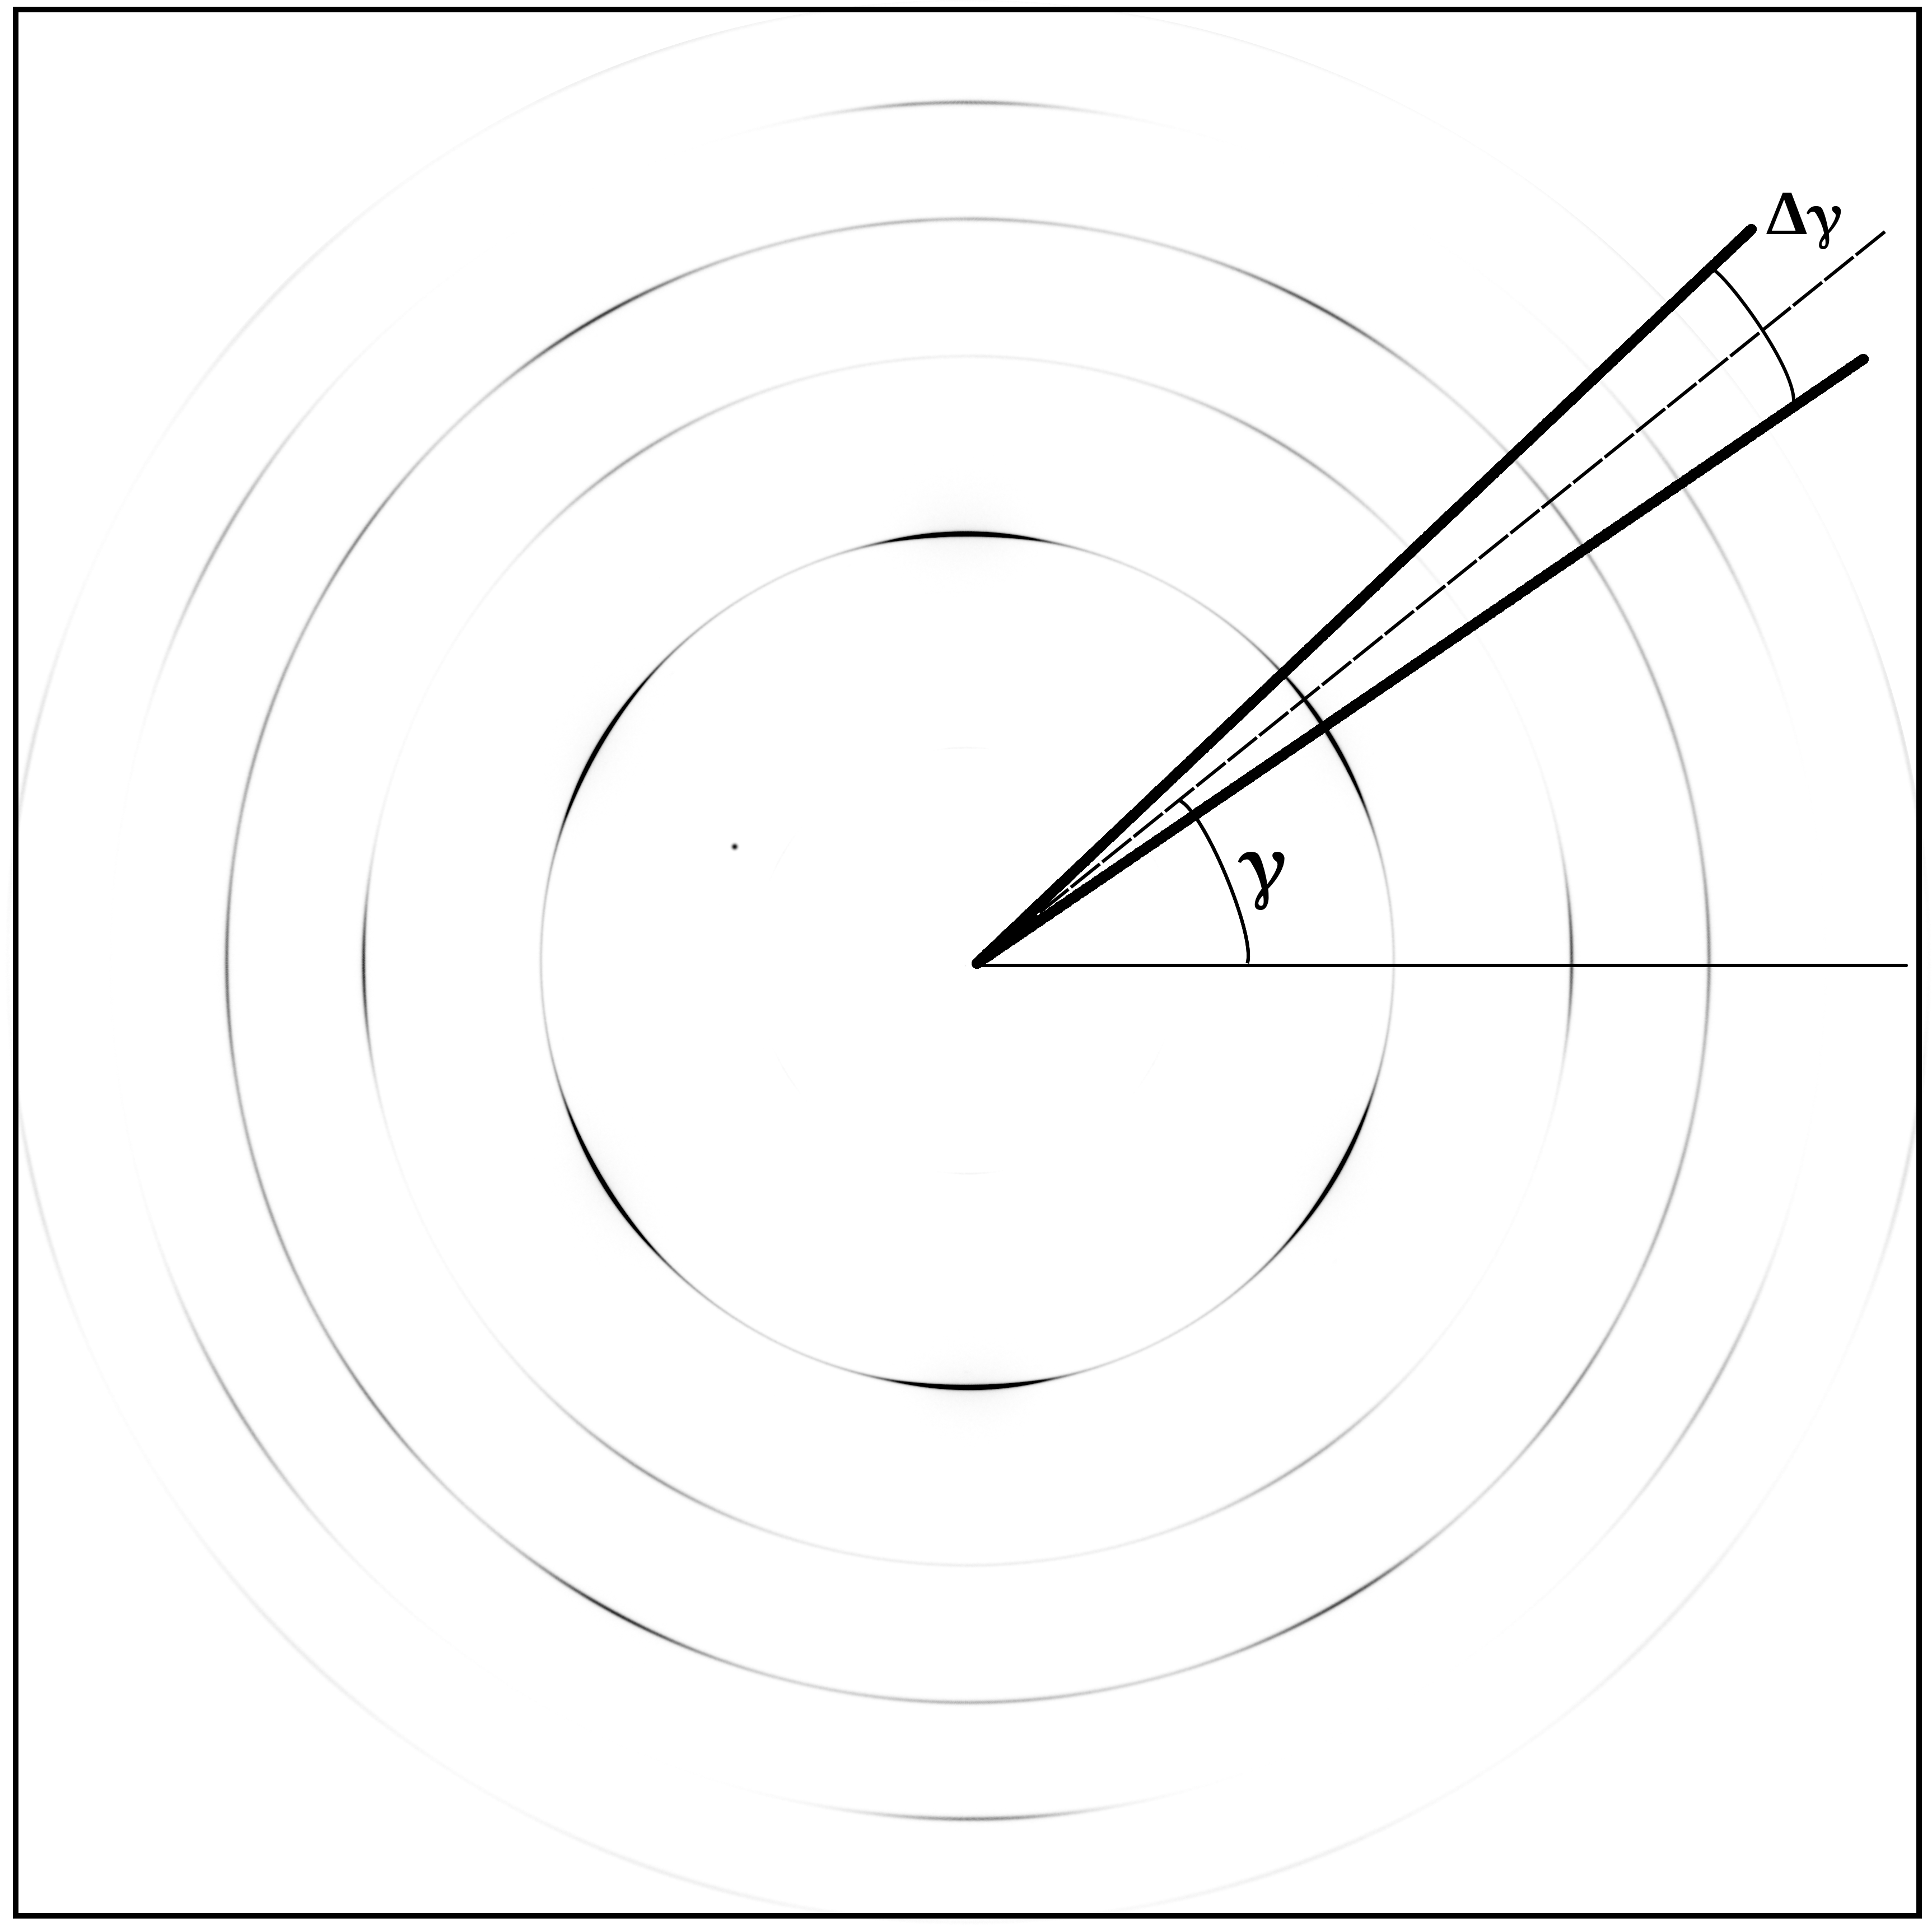
\includegraphics[width=0.5\textwidth]{Fit2D_2}
  \caption{Para convertir las imágenes grabadas en cada experimento de difracción se empleó el programa FIT2D, que permitió dividir a cada conjunto de anillos de Debye en 72 porciones de 5\,$^{\circ}$ cada una. El programa luego extraía la intensidad de promedio grabada dentro de cada porción y con esa información construía difractogramas que fueron luego empleado para realizar los ajustes.}
  \label{fig:fit2d}
\end{figure}

Una vez obtenidos todos los difractogramas, los mismos fueron tratados con un software de elaboración propia, tanto para aplicar el método de Langford como el CMWP.

Ambos software toman como dato de entrada todos los difractogramas obtenidos con FIT2D, además de otros archivos que deben ser escritos por el usuario, y que se encuentran ejemplificados en el apéndice \ref{CA:input}.

En el caso del programa que realiza el análisis de Langford se precisan tres archivos además de los datos extraídos de FIT2D.
El primero se denomina \hyperlink{datainfo}{data\_info\_1.ini} y contiene la información que indica dónde se guardarán los resultados y dónde se encuentran los archivos de entrada, así como su cantidad y los datos necesarios para realizar la conversión angular.
También la resolución en píxeles del detector y la distancia entre el detector y la muestra, datos necesarios para convertir las distancias sobre el detector a la variable 2$\theta$.
La opción \textit{Treshold} es un dato numérico que se emplea para determinar cuál es la intensidad mínima por encima del ruido de fondo que debe tener un pico para ser ajustado por el método de mínimo cuadrados. 
Como ajustar picos de baja intensidad puede llevar a alargar el tiempo que lleva procesar los datos, además de dar resultados poco confiables, no se recomienda colocar 0 como valor de umbral, mientras que un valor de 5 ha dado buenos resultados para las mediciones realizadas en esta tesis, como se puede ver en la Fig. \ref{fig:MinIntensity}

\begin{figure}[!htb]
  \centering
  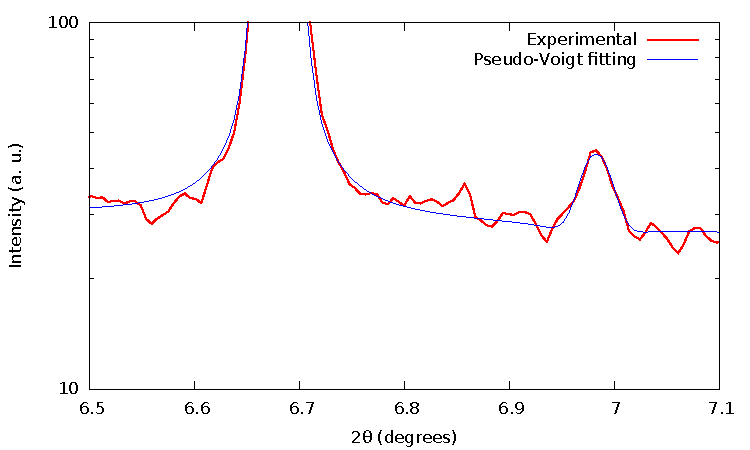
\includegraphics[width=0.8\textwidth]{Pico_minimo}
  \caption{La relación señal ruido mínima que permite distinguir y ajustar apropiadamente un pico del difractograma. El pico que se muestra tiene una intensidad integrada neta de 5 y como puede verse es ajustado razonablemente por una función pseudo-Voigt. Si el pico es más pequeño el error del ajuste se vuelve muy grande e incluso puede no converger.}
  \label{fig:MinIntensity}
\end{figure}

Las banderas \textit{Printpattern} y \textit{Correctwitdh} determinan si se van a imprimir los difractogramas extraídos junto con el mejor ajuste de cada uno, y si se van a realizar correcciones sobre el ancho de pico teniendo en cuenta el ancho de la muestra.
Esta es una característica experimental al momento de la escritura de la tesis, y debe emplearse con mucho cuidado.
Finalmente, también debe indicarse la cantidad de picos que se desean ajustar, junto con una coordenada aproximada de su centro (en 2$\theta$), los píxeles que definen inicio y final de cada pico, y dos píxeles que se determinarán el valor del ruido debajo de cada pico.

En el archivo \hypertarget{fitini}{\textit{fit\_ini\_2.ini}} debe indicarse nuevamente la cantidad de picos a ajustar, así como la cantidad de puntos de ruido que se ajustarán en la rutina de mínimos cuadrados.
La rutina de mínimos cuadrados minimiza la suma total de la diferencia entre las intensidades experimentales $I_{exp}$ y las intensidades teóricas $I_{teor}$ dadas por una suma de funciones pseudo-Voigt (Ec. \ref{eq:pseudovoigt}), una por cada pico, además de un ruido que se modela como una función lineal por partes, con $N_{ruido}$ partes, cantidad que es definida por el usuario:
\begin{equation}
  I_{teor} \ = \sum_{i=1}^{N_{picos}} \ pV_i (2\theta; \ I_{0i}, 2\theta_{B_i}, H_{gl}, \eta_{gl}, H_i^{part}, \eta_i^{part}) \ + \sum_{j=0}^{N_{ruido}} Bg(2\theta; \ I_{B_j}, I_{B_{j+1}})
  \label{eq:Iteor}
\end{equation}
\noindent
donde la función ruido $Bg(2\theta)$ es una función lineal dentro de un intervalo definido por $2\theta_j$ y $2\theta_{j+1}$ definido por el usuario y cero fuera de ese intervalo.
La función de ruido tiene intensidad $I_j$ en el punto $2\theta_j$ e intensidad $I_{j+1}$ en el punto $2\theta_{j+1}$, y las intensidades $I_j$ e $I_{j+1}$ son ajustadas dentro de la rutina de mínimos cuadrados.
De las funciones $pV(x)$, de las que hay una por pico, se ajusta su intensidad integrada $I_{0i}$, su centro $2\theta_{Bi}$ y su ancho y factor de mezcla.
El FWHM y el factor de mezcla de cada pico se generan a partir de un valor global (el mismo para todos los picos) y uno particular que se ajustan en pasos distintos del algoritmo de ajuste:

\begin{align}
  H_i & = H_{gl} \ + \ H_i^{part} \nonumber \\
  \eta_i & =  \eta_{gl} \ + \ \eta_i^{part}
  \label{eq:global}
\end{align}
\noindent
El motivo de esta separación es pura y exclusivamente por cuestiones de estabilidad numérica durante el ajuste, y no tiene una razón física detrás.

Todos los valores son ajustados por un rutina de mínimos cuadrados que emplea el algoritmo de Levenberg-Marquardt\cite{wiki:Levenberg} para minimizar el argumento de mínimos cuadrados:
\begin{equation}
  S(\mathbf{\chi}) \ = \ \sum_{i=1}^{N} (I^{exp}_i - I^{teor}_i(\mathbf{\chi}))^2
  \label{eq:argmin}
\end{equation}
\noindent
donde $\mathbf{\chi}$ es el conjunto de todos los parámetros que se varían para determinar la curva teórica que da el mejor ajuste a los datos experimentales.
Como el ajuste se realiza sobre cada difractograma en forma individual, $N$ indica la cantidad de mediciones que hay en un dado difractograma.

Una vez realizado el ajuste sobre todos los difractogramas, se toma la información de cada pico, el conjunto $(\theta_B, \ I_0, \ H, \ \eta)$ que tiene asociadas las coordenadas en el sistema de laboratorio $(\omega, \ \gamma, \ \theta_B)$ y se les asigna las coordenadas  $(\alpha, \ \beta)$ en el sistema de referencia del cristal, y con esos datos se construyen las figuras de polos y las figuras de polos generalizadas.
Antes de imprimir la salida de los archivos, el software substrae el ancho instrumental a partir de los valores que están presentes en el archivo \hyperlink{IRF}{\textit{IRF\_3.dat}}.
Las substracción de los datos se hace suponiendo que el ancho instrumental tiene una componente Gaussiana y una componente Lorentziana, y que ambas crecen con el ángulo $\theta$ siguiendo la ley de Caglioti\cite{Caglioti1958}:
\begin{align}
  \left[H_{ins}^{G}\right]^2 & =  U_G \ \tan^2(\theta) \ + \ V_G \ \tan(\theta) \ + \ W_G \nonumber \\
  H_{ins}^{L} & =  U_L \ \tan^2(\theta) \ + \ V_L \ \tan(\theta) \ + \ W_L
  \label{eq:caglioti}
\end{align}
\noindent
donde los parámetros $(U_i, V_i, W_i)$ deben ser especificados por el usuario.
En el archivo \textit{IRF\_3.dat} también deben especificarse los parámetros geométricos de la muestra para tener en cuenta la contribución del ancho de la muestra al ensanchamiento de los picos.

Los datos así obtenidos fueron procesados y graficados utilizando MTEX\cite{Hielscher2008}, un paquete de Matlab para el procesamiento de texturas.

El software que realiza el ajuste utilizando el método CMWP, tiene dos etapas básicamente: en la primera hace un ajuste al difractograma con una función como la mostrada en la Ec. \ref{eq:Iteor}, y siguiendo la metodología descripta anteriormente usa los resultados del ajuste para generar una serie de archivos auxiliares que se necesitan para la segunda etapa.
En la segunda etapa corre en forma automática el programa CMWP siguiendo una estrategia de ajuste determinada por el usuario.

Como la primera parte de este programa funciona con un objetivo similar al del programa anterior, el primer archivo de entrada, denominado \hyperlink{dinfoCMWP}{\textit{data\_info\_1.ini}} es casi igual al del programa anterior, con la diferencia de que al especificar la posición de los picos a ajustar se pide que se indique un número de fase que empieza en 0, ya que este es un dato necesario para el programa CMWP.

El segundo archivo se llama \hyperlink{fitstrategy}{\textit{fit\_strategy\_2.ini}} el usuario deber indicar los parámetros iniciales para el ajuste con pseudo-Voigts, como con el programa anterior, pero además deber indicar cuántos pasos de ajuste desea realizar con el programa CMWP, y cuáles son los coeficientes que va a ajustar en cada paso.
También debe indicar si desea que el CMWP haga un ajuste por fallas de apilamiento  y si desea que se ajuste independientemente la intensidad y posición de los picos.
En la práctica se ha visto que hacer un ajuste extra de intensidades alarga mucho el tiempo de cálculo del programa y no aporta valores finales muy diferentes a los que se obtienen cuando no se hace este ajuste.

Los siguientes tres archivos que debe generar el usuario son llamados archivos \textit{plantilla}, ya que estos archivos no suelen escribirse a mano, sino que son generados por el programa CMWP automáticamente, como ya se explicó en la Sec \ref{SS:CMWP}.


\iffalse
\subsection{Langford}\label{SS:MLgfrd}

\begin{figure}[!htb]
  \centering
  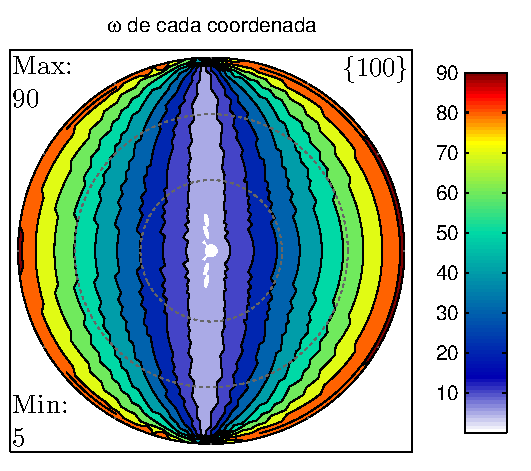
\includegraphics[width=0.8\textwidth]{Conv_PF_omega_contourf}
  \caption{Relación entre las coordenadas angulares y las coordenadas de las figuras de polos.}
  \label{fig:LabtoPF}
\end{figure}

\begin{figure}[!htb]
  \centering
  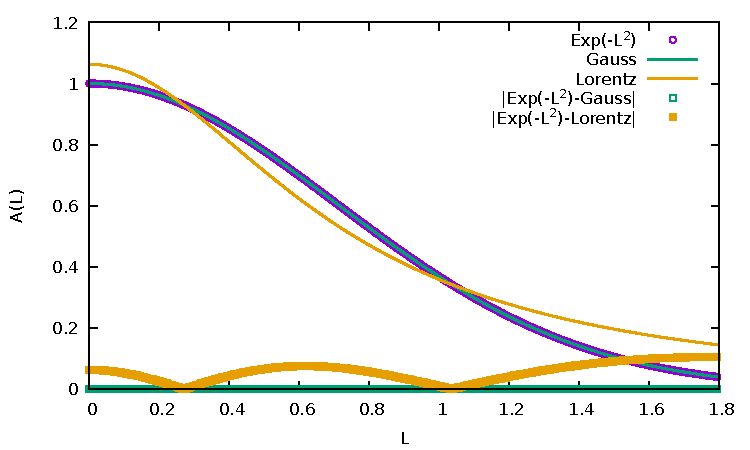
\includegraphics[width=0.8\textwidth]{GaussianStrain}
  \caption{Coeficientes de strain gaussiano y lorentziano.}
  \label{fig:GaussStrainn}
\end{figure}

\begin{figure}[!htb]
  \centering
  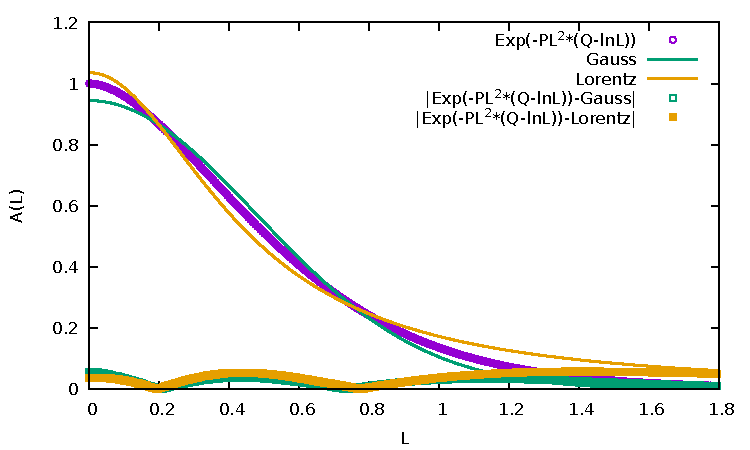
\includegraphics[width=0.8\textwidth]{RealStrain}
  \caption{Coeficientes de strain posta.}
  \label{fig:RealStrain}
\end{figure}

\begin{figure}[!htb]
  \centering
  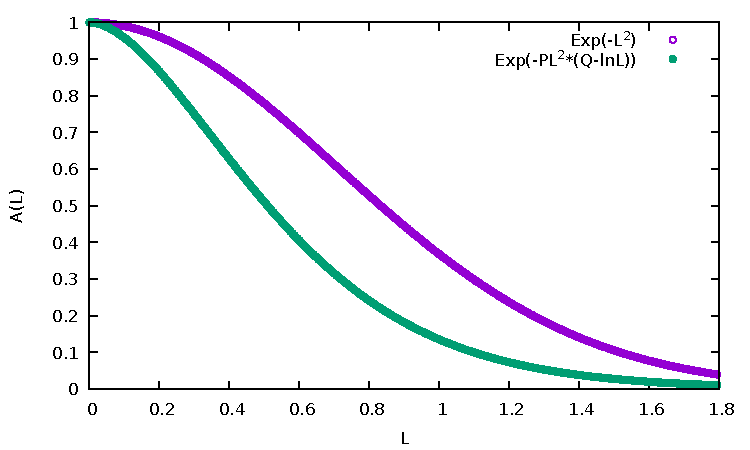
\includegraphics[width=0.8\textwidth]{Strain_Compare}
  \caption{Comparacion del gaussiano con el posta.}
  \label{fig:RealvsGauss}
\end{figure}

\newpage
\fi
\section{Mediciones de EBSD}\label{S:MatEBSD}
Los métodos de determinación de micro-estructura empleando difracción de rayos X tienen la ventaja de permitir estudiar propiedades volumétricas del material con una estadística más que razonable.
Sin embargo, dado que los estudios de ancho de pico son métodos indirectos que requieren la resolución de un problema matemáticamente mal planteado, en el transcurso de esta tesis fue necesario complementar los resultados obtenidos con mediciones de EBSD, que permite hacer una determinación más directa de ciertas características micro-estructurales, sobre todo aquellas que tienen que ver con la orientación de los cristales en el material.
Entre éstas se encuentran la textura cristalográfica, los tamaños de dominio y la deformación acumulada.

Las mediciones de EBSD fueron realizadas en el microscopio electrónico de barrido (SEM, por sus siglas en inglés) instalado en CCT Rosario - Laboratorio de Microscopía Electrónica de Barrido.
El mismo es un microscopio FEI Quanta 200E con cañón emisor de efecto de campo, detector de electrones secundarios y retro-dispersados, con capacidad de trabajar en alto y bajo vacío y en condiciones ambientales (ESEM) y detector de EBSD (Ver Fig. \ref{fig:SEM}).
El software de adquisición empleado es TSL OIM Data Collection 5, para el análisis de los datos se emplearon los programas OIM TSL 7.3 y MTEX.

\begin{figure}[!htb]
  \centering
  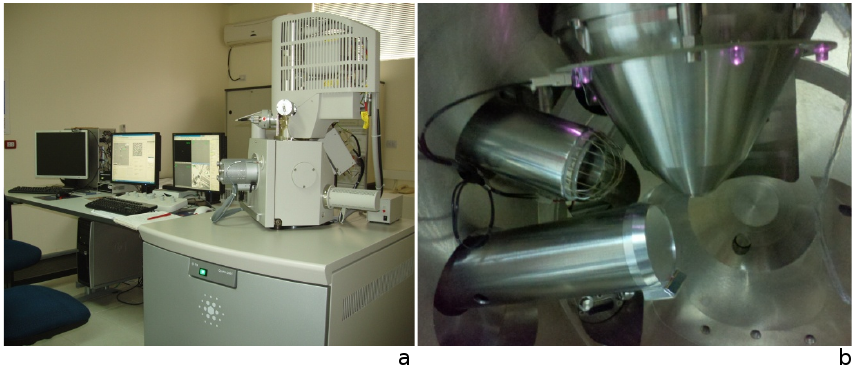
\includegraphics[width=\textwidth]{SEM}
  \caption{Fotografías del microscopio electrónico de barrido FEI Quanta 200E ubicado en el CCT Rosario - Laboratorio de Microscopía Electrónica de Barrido. (a) Vista externa del microscopio y computadoras para adquisición, análisis y soporte. (b) Imagen del interior del microscopio, donde se pueden apreciar el cañón emisor y los detectores.}
  \label{fig:SEM}
\end{figure}

La preparación de las muestras para este instrumento fue bastante diferente a la utilizada para difracción de rayos X, ya que dado que la técnica de EBSD es esencialmente superficial es preciso reducir la rugosidad de la superficie estudiada para obtener patrones de Kikuchi lo más nítidos que sea posible.
Además, como el haz de electrones no incide perpendicularmente sobre la muestra sino que lo hace con un ángulo de 70\,$^{\circ}$, cualquier rugosidad en la muestra producirá ``sombras'' en el haz de electrones, lo que producirá una distorsión artificial en la microestructura observada.
El pulido sobre las muestras cortadas inicia con papel de lija, como en la preparación para los experimentos de XRD, pero continúa con un pulido con pasta de diamante de 9, 6, 3 y 1\,$\mu$m, en ese orden, finalizando con un pulido con sílica coloidal de 0.05\,$\mu$m.
Finalmente, la muestra se incluye en resina conductora, lo que permite conectar la muestra a tierra, evitando que se acumulen cargas eléctricas que puedan impedir obtener una imagen nítida.

Para determinar la textura del material con EBSD y poder compararla con la medida a través de XRD, es preciso hacer barridos de gran área para aumentar la estadística, lo que obliga a reducir la resolución del barrido para reducir el tiempo de barrido y de post-procesamiento.
Para los materiales estudiados, los barridos realizados para la determinación de textura se realizaron sobre áreas del orden de 600\,$\mu$m (RD) x 500\,$\mu$m (ND/TD) con una resolución de 0.4\,$\mu$m.
Se eligió que la dirección más larga del barrido sea siempre RD, ya que como la mayoría de los materiales estudiados fueron laminados, se esperaba que los granos fueran más largos en la dirección que laminado que en cualquiera de las direcciones perpendiculares.

El análisis de la anisotropía en la deformación acumulada y en el tamaño de grano se realizó sobre mapas con menor área y mayor resolución, ya que los detalles de la micro-estructura de los materiales deformados se pierden a resoluciones bajas.
Por ejemplo, si en un material deformado se espera tener granos de tamaño del orden de pocos micrones, o incluso de algunos nanómetros, si la resolución es de 0.4\,$\mu$m se cometer el error de asignar múltiples granos a un solo píxel.
Por lo tanto, los barridos realizados para obtener detalles de la micro-estructura se realizaron sobre áreas de 250\,$\mu$m (RD) x 80\,$\mu$m (ND/TD) con una resolución de 0.1\,$\mu$m.
Como se explicó en el párrafo anterior, fue preciso aumentar la longitud estudiada en la dirección de laminado de las muestras por la morfología que se esperaba observar en los granos de los materiales estudiados.

En esta tesis no se aplicaron métodos de “clean-up” para limpiar los datos ya que los puntos de los barridos con bajo índice de calidad corresponden a las zonas de alta deformación del material, y son precisamente estas zonas las que se intentan estudiar en esta tesis. 
Eso exigió un trabajo especial en obtener superficies adecuadas con la calidad necesaria para que la indexación sea la adecuada en una gran proporción de los puntos inspeccionados.

La determinación de la textura en las mediciones de EBSD es un proceso directo, ya que se mide la orientación de los cristales.
En el caso de MTEX, el cálculo de la ODF se hace a partir del desarrollo en serie de las llamadas funciones radialmente simétricas $\psi_L$:

\begin{equation}
  f(g) \ \sim \ \sum_{l=0}^{L} \sum_{k,k'=-l}^{l} \ \hat{f}(l, k, k') \ \psi_L(\omega(gg_i)) 
  \label{eq:ODFEBSD}
\end{equation}
\noindent
donde los coeficientes $\hat{f}$ del desarrollo \ref{eq:ODFEBSD} se calculan directamente a partir de las $N$ orientaciones $g_i$ medidas en el experimento de EBSD:
\begin{equation}
  \hat{f}(l, k, k') \ = \ \frac{1}{N} \ \frac{(l + 1/2)^{1/2}}{2 \pi} \sum_{i=1}^{N} \overline{T_l^{k k'} (g_i)}; \quad l \leq L, \ k, k' = -l, \cdots, l
  \label{eq:ODFcoef}
\end{equation}
\noindent
donde $T_l^{k k'}$ son los armónicos esféricos generalizados, y la barra denota conjugación compleja. Las funciones $\psi_L$ representan orientaciones ideales en el espacio de orientaciones $SO(3)$ y son funciones de distribución que tienen su máximo cuando $g \ = \ g_i$ y decrecen monótonamente a medida que aumenta el ángulo $\omega$ entre $g$ y $g_i$.
Las funciones radialmente simétricas tienen asociado un ancho de de banda que se denota $\kappa$, que determina que tan intensa va a ser la textura alrededor de la orientación $g_i$.
A mayor $\kappa$, la distribución se vuelve más ancha y la textura menos intensa.

En teoría, el desarrollo \ref{eq:ODFEBSD} tiene infinitos términos, sin embargo por cuestiones de cómputo la serie se trunca en el $L$-ésimo término, que debe incrementarse para texturas muy intensas, es decir, en la medida que se quiera determinar una ODF muy intensa, el desarrollo en serie debe truncarse para $L$'s cada vez mayores, lo cual se logra reduciendo el parámetro $\kappa$ que condiciona el ancho de las funciones $\psi_L$.

La determinación de tamaño de grano en EBSD es conceptualmente distinta a los métodos análogos que se emplean en XRD o incluso en la metalografía tradicional.
Mientras que en XRD se obtiene una longitud promedio de las columnas cristalinas que difractan coherentemente en una dada dirección, en los análisis de EBSD el concepto de grano se define a partir de regiones cerradas que poseen una mis-orientación menor que cierto valor umbral definido por el usuario.
En general, y salvo que se especifique lo contrario, dos píxeles se considerarán en diferentes granos si su mis-orientación es mayor a 5\,$^{\circ}$, que es el criterio que se emplea normalmente en los análisis de EBSD.

La determinación de la deformación de la deformación acumulada en el material se hizo a partir del cálculo de las dislocaciones geométricamente necesarias (GND, por sus siglas en inglés).
El cálculo de las GND se hace a partir de calcular el tensor de Nye\cite{Nye1953}, que se calcula a partir de la curvatura de la red cristalina, que a su vez puede obtenerse a partir de medir la mis-orientación entre celdas vecinas\cite{Pantleon2008}.
La curvatura de la red cristalina se calcula midiendo la mis-orientación entre un dado píxel y sus vecinos en un dado mapa de EBSD, dejando afuera aquellos píxeles que pertenezcan a granos diferentes.
Debe notarse además que píxeles con una mis-orientación menor a los 0.5\,$^{\circ}$ tendrán una mis-orientación nula, ya que esa es la incerteza que se comete al medir mis-orientaciones con un microscopio como el empleado en este trabajo.

\chapter{Estudio sobre el acero libre de intersticiales}
\graphicspath{{./figs/03_IF/}}
\chapterquote{The void is without substance but cuts lile steel.}
\section{Estudio de la microestructura por el método CMWP}\label{S:IFCMWP}
\section{Estudio de la microestructura por el método de Langford y figuras de polos generalizadas}\label{S:IFLANG}
\section{Estudio de la microestructura por EBSD}\label{S:IFEBSD}
\section{Discusión de resultados}\label{S:IFDis}
\section{Conclusiones}\label{S:IFConclusiones}

\chapter{Estudio sobre el acero F138}
\graphicspath{{./figs/04_F138/}}
\section{Estudio de la microestructura por el método CMWP - Revisión}\label{S:F138CMWP}
\section{Estudio de la microestructura por el método de Langford y figuras de polos generalizadas}\label{S:F138LANG}
\section{Estudio de la microestructura por EBSD - Revisión}\label{S:F138EBSD}
\section{Discusión de resultados}\label{S:F138Dis}
\section{Conclusiones}\label{S:F138Conclusiones}

%\chapter{Estudio sobre el acero duplex G2205}
\graphicspath{{./figs/06_G2205/}}
\section{Estudio de la microestructura por el método de Langford y figuras de polos generalizadas}\label{S:G2205LANG}
\section{Discusión de resultados}\label{S:G2205Dis}
\section{Conclusiones}\label{S:AlConclusiones}

\chapter{Estudio sobre el Aluminio 1050}
\graphicspath{{./figs/06_Al/}}
\section{Estudio de la microestructura por el método CMWP}\label{S:AlCMWP}
\section{Estudio de la microestructura por el método de Langford y figuras de polos generalizadas}\label{S:AlLANG}
\section{Estudio de la microestructura por EBSD - Revisión}\label{S:AlEBSD}
\section{Discusión de resultados}\label{S:AlDis}
\section{Conclusiones}\label{S:AlConclusiones}

\chapter{Estudio sobre el Aluminio 1050 laminado asimétricamente}\label{C:AlA}
\graphicspath{{./figs/07_AlA/}}
\section{Estudio de la microestructura por el método de Langford y figuras de polos generalizadas}\label{S:AlALANG}
Recristalizado. Algún dato de CMWP
Uso el otro aluminio

\section{Discusión de resultados}\label{S:AlDis}
\section{Conclusiones}\label{S:AlConclusiones}

%\chapter{Conclusiones}\label{C:Conclusiones}

%\chapter{Proyecciones}\label{C:Proyecciones}


\appendix
\chapter{Archivos de entrada utilizados para correr los programas empleados en el desarrollo de esta tesis}\label{CA:input}
%\chapterquote{Negociemos Don Inodoro}{Fernando de la R\'{u}a, 2001}
%\chapterquote{Smartness runs in my family.  When I went to school I was so smart my teacher was in my class for five years}{George Burns}
\graphicspath{{figs/Apendice}}
En las secciones siguientes se muestran archivo de ejemplo de los archivos de entrada necesarios para la ejecución de los programas empleados en el transcurso de esta tesis.
El detalle acerca del flujo de trabajo puede encontrarse en el capítulo \ref{C:Materiales}, y al final del nombre de cada archivo figura un número que indica el orden en que debe ingresarse cuando se corre el programa.
\section{Datos de entrada de IDEA}
\subsection{Archivo \textit{data\_info\_1.ini}}
\begin{lstlisting}[language=Python]
1.PathForOutput     : /path/to/output/
2.NrOfSamples(1)    : 1

Input Data - 1
3.InputFilePath     : /path/to/spr/files/
4.InputFileName     : New_Al70R-tex_
5.FileExtension     : spr
6.IndexNr Start     : 1
7.Start Angle       : 1
8.IndexNr End       : 1
9.End Angle         : 1
10.DeltaIndexNr     : 1
11.Delta Angle      : 5
12.Start Gamma      : 0
13.End Gamma        : 359
14.Delta Gamma      : 5
15.Distance (mm)    : 1081
16.Pixel value (mm) : 0.1
17.Treshold         : 5
18.Printpattern(y/n): y
19.Correctwidth(y/n): y

Peak Positions
I. NrOfPeaks        : 7
II. Peak Positions
(2Theta Peak-L Peak-R BG-L BG-R):
1.742 583 713 400 935
2.013 713 854 500 965
2.850 1025 1130 965 1178
3.342 1215 1298 1190 1450
3.489 1298 1375 1190 1450
4.025 1505 1559 1450 1600
4.391 1650 1685 1620 1700
\end{lstlisting}


\subsection{Archivo \textit{fit\_ini\_2.ini}}
\begin{lstlisting}
#FIT_INI: archivo con las estimaciones de los valores iniciales para el ajuste
#Peaks   Bg
7       19
#Global_H:
0.04500   
#Global_eta:
0.4400     
#2theta0    I0    shift_H    shift_eta
3.4840     2.0   0.0000     0.00000 
4.0240    64.0   0.0000     0.00000
5.6959    25.0   0.0000     0.00000
6.6794    17.0   0.0000     0.00000
6.9757     1.0   0.0000     0.00000
8.0569     6.0   0.0000     0.20000
8.7843     1.0   0.0000     0.50000
#Bg_pos(2theta) Bg_int
0.000       28.0050
0.360       28.0050
0.560       28.0050
0.880       28.0050
1.250       28.0050
2.050       44.8004
2.119       28.0050
2.648       28.0050
3.060       29.1600
4.369       34.2893
4.943       28.0050
5.048       25.1649
5.101       28.0050
6.219       28.0050
6.282       28.0050
7.640       28.0050
8.419       28.0050
8.523       28.0050
8.937       28.0050
\end{lstlisting}

\subsection{Archivo \textit{IRF\_3.dat}}
\begin{lstlisting}
# Instrumental broadening
UG: 0.0108706
VG: 0.0010735
WG: 0.0002242
UL: 0.0499984
VL: 0.0104957  
WL: 0.0037801

# Sample information
Cilinder(c)/Rect.(r):  r
Lenght@omega=0  (mm):  1.0
Lenght@omega=90 (mm):  2.0
Absorption (1/cm):     3.0
\end{lstlisting}
%%%%%%%%%%%%%%%%%%%%%%%%%%%%%%%%%%%%%%%%%%%%%%%%%%%%%%%%%%%%%%%%%%%%%%%%
\section{Datos de entrada de IDEA-CMWP}
\subsection{Archivo \textit{data\_info\_1.ini}}
\begin{lstlisting}
File Input Data
1.PathForSPR        : /home/ebenatti.ifir/CMWP/CMWP-140518/data/G2205/00/spr/
2.PathForOutput     : data/G2205/
3.InputFileName     : G2205-0-tex_
4.PathForBaseFiles  : /home/ebenatti.ifir/CMWP/CMWP-140518/data/G2205/
5.NameOfBaseFiles   : G220500
6.PathResultsFolder : /home/ebenatti.ifir/CMWP/CMWP-140518/results/evaluate-int-dir/
7.FileExtension     : spr
8.IndexNr Start     : 1
9.DeltaIndexNr      : 1
10.IndexNr End      : 37
11.Start Angle      : 0
12.Delta Angle      : 5
13.End Angle        : 180
14.Start Gamma      : 0
15.Average Gamma    : 5
16.Delta Gamma      : 5
17.End Gamma        : 359

IDEA Input Data
17.Distance         : 1081e-3
18.Pixel value      : 100e-6
19.Treshold         : 4

Peak Positions
I. NrOfPeaks        : 9
II. NrOfPhases      : 2
III. Peak Positions
ph hkl 2Theta Peak-L Peak-R BG-L BG-R:
0 111 3.963 745 754 700 820
1 110 4.052 758 774 700 820
0 200 4.575 856 874 820 900
1 200 5.711 1073 1089 1040 1110
0 220 6.445 1213 1231 1180 1250
1 211 6.983 1318 1332 1280 1350
0 311 7.547 1424 1442 1390 1460
0 222 7.877 1490 1501 1470 1510
1 220 8.052 1521 1539 1510 1560
\end{lstlisting}

\subsection{Archivo \textit{fit\_strategy\_2.ini}}
\begin{lstlisting}
#FIT_INI: seeds of the fitting and fitting strategy
#Global_H:
0.03000   
#Global_eta:
0.4600     
#2theta0    I0    shift_H    shift_eta
4.0520    22.07  0.0000     0.00000 
5.7210   122.46  0.0000     0.00000
6.9970    90.69  0.0000     0.00000
8.0700     1.70  0.0000     0.00000
# Fitting strategy
# Ajustar intensidades (y/n)?
n
# Ajustar por fallas de apilamiento (y/n)?
n
# Numero de pasos de ajuste
1
# fix.a fix.b fix.c fix.d fix.e fix.stpr fix.de
1   y     n     y     n     y     y        y
2   y     y     n     y     n     y        n
3   n     n     y     y     y     y        y
4   y     n     y     n     y     y        y
5   y     y     n     y     n     y        n
6   n     n     y     y     y     y        y
\end{lstlisting}

Los siguientes archivos son creados automáticamente por el programa CMWP y no sería necesario crearlos, pero se muestran en esta sección por completitud.
\subsection{Archivo \textit{sample.dat.ini} (CMWP)}
\begin{lstlisting}
la=0.405
bb=0.286378
C0=0.15
wavelength=0.014267
\end{lstlisting}

\subsection{Archivo \textit{sample.dat.fit.ini} (CMWP)}
\begin{lstlisting}
init_a=4.64921
init_b=3.42161
init_c=0.272639
init_d=1.8779
init_e=4.2515
init_epsilon=1.0
d_fixed="y"
e_fixed="y"
scale_a=1.0
scale_b=1.0
scale_c=1.0
scale_d=1.0
scale_e=1.0
\end{lstlisting}

\subsection{Archivo \textit{sample.dat.q.ini} (CMWP)}
\begin{lstlisting}
USE_SPLINE=y
NO_SIZE_EFFECT=n
SF_ELLIPSOIDAL=n
INDC=n
USE_STACKING=n
USE_WEIGHTS=y
WEIGHTING_ALGORITHM=1
peak_int_fit=n
peak_pos_fit=n
fit_in_K=n
DISABLE_COINC_G2=n
ENABLE_CONVOLUTION=n
IF_TH_FT_limit=1e-12
PROF_CUT=10
N1=1024
N2=1024
minx=3.0
maxx=8.95
FIT_LIMIT=1e-12
FIT_MAXITER=1000
NUMBER_OF_PHASES=1
FIT_ONLY_PHASE=0
\end{lstlisting}

\begin{biblio}
  \bibliography{./bib/tesis_lib,./bib/Physical_Properties_of_Crystals,./bib/International_Tables_for_Crystallography}
\end{biblio}

\begin{postliminary}

\listoffigures                  %Figuras

\listoftables                   %Tablas

\listofabbr                     %Símbolos y abreviaturas

%\begin{seccion}{Publicaciones asociadas}
%  \begin{enumerate}
%  \item Mi primer aviso en la revista \textbf{ABC}, 1996
%  \item Mi segunda publicaci\'{o}n en la revista \textbf{ABC}, 1997
%  \end{enumerate}
%\end{seccion}

\end{postliminary}

\end{document}
